% Created by tikzDevice version 0.12.6 on 2026-08-01 05:44:19
% !TEX encoding = UTF-8 Unicode
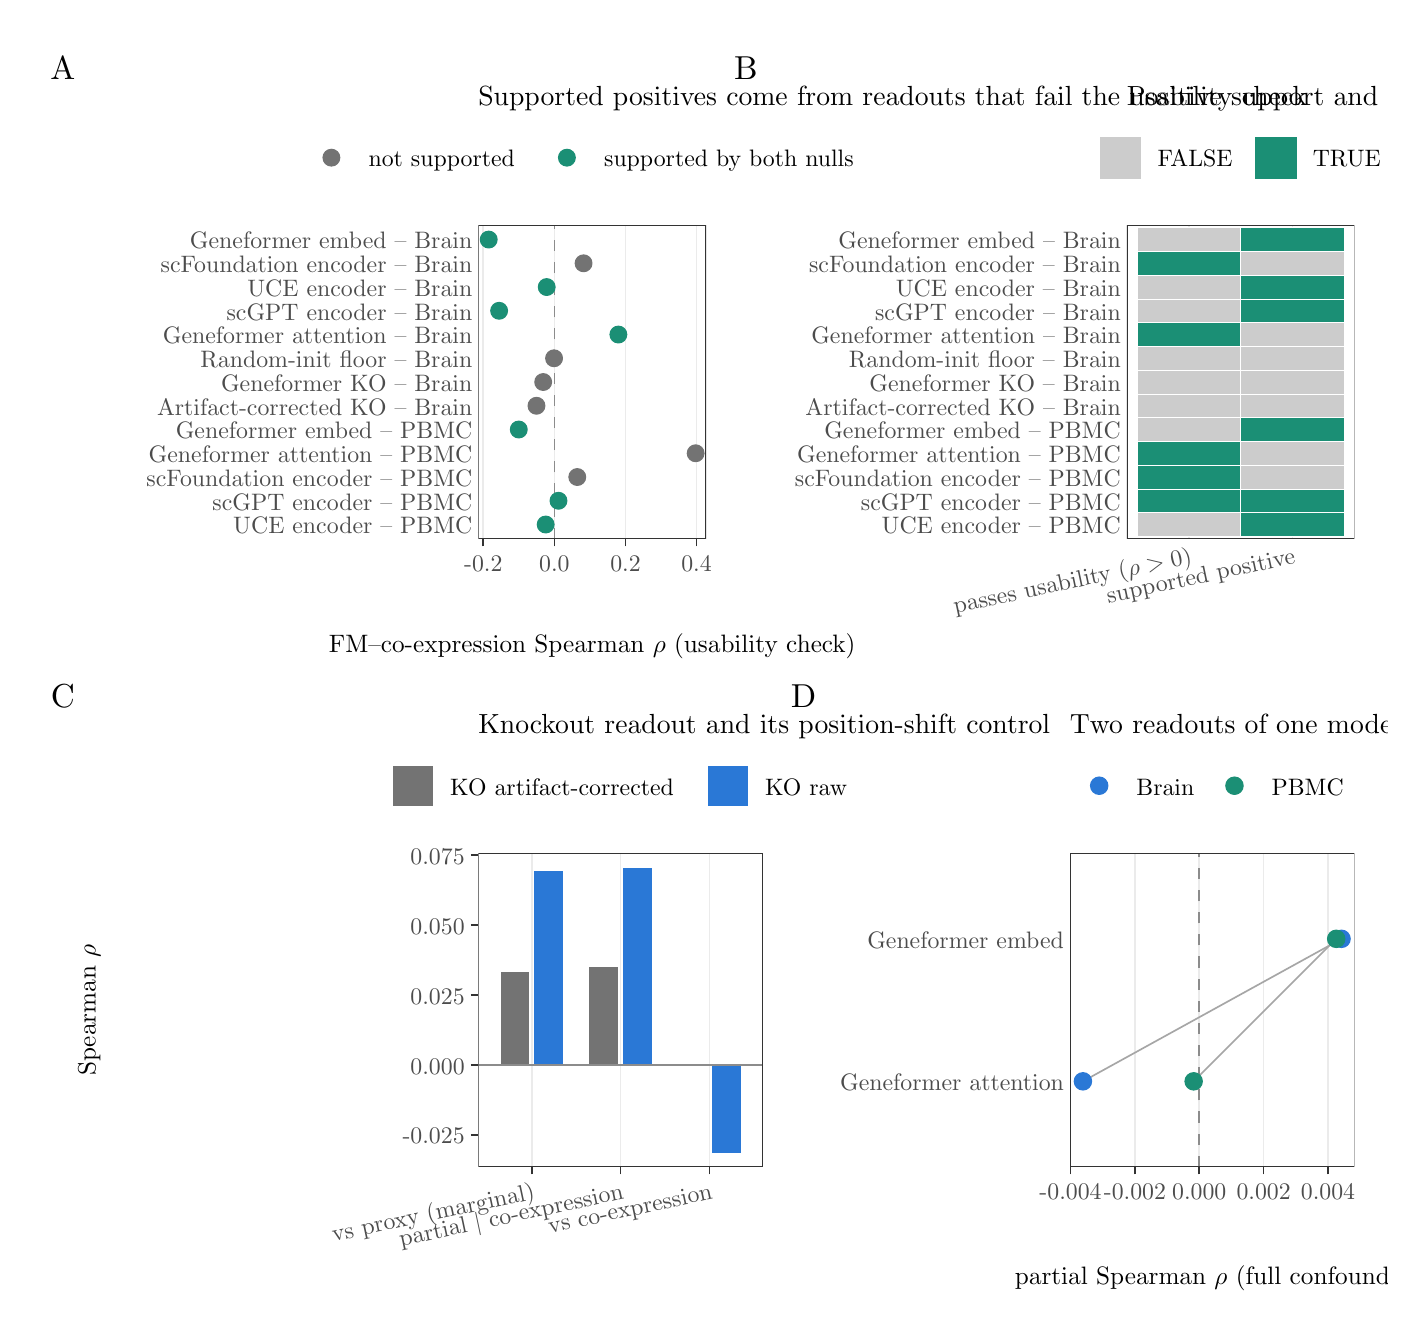
\begin{tikzpicture}[x=1pt,y=1pt]
\definecolor{fillColor}{RGB}{255,255,255}
\path[use as bounding box,fill=fillColor,fill opacity=0.00] (0,0) rectangle (491.44,462.53);
\begin{scope}
\path[clip] (  0.00,  0.00) rectangle (491.44,462.53);
\definecolor{drawColor}{RGB}{255,255,255}
\definecolor{fillColor}{RGB}{255,255,255}

\path[draw=drawColor,line width= 0.6pt,line join=round,line cap=round,fill=fillColor] (  0.00,  0.00) rectangle (491.44,462.53);
\end{scope}
\begin{scope}
\path[clip] (  4.00,231.59) rectangle (251.11,458.53);
\definecolor{drawColor}{RGB}{255,255,255}
\definecolor{fillColor}{RGB}{255,255,255}

\path[draw=drawColor,line width= 0.6pt,line join=round,line cap=round,fill=fillColor] (  4.00,231.59) rectangle (251.11,458.53);
\end{scope}
\begin{scope}
\path[clip] (251.11,231.59) rectangle (485.44,458.53);
\definecolor{drawColor}{RGB}{255,255,255}
\definecolor{fillColor}{RGB}{255,255,255}

\path[draw=drawColor,line width= 0.6pt,line join=round,line cap=round,fill=fillColor] (251.11,231.59) rectangle (485.44,458.53);
\end{scope}
\begin{scope}
\path[clip] (162.86,277.85) rectangle (245.11,391.10);
\definecolor{fillColor}{RGB}{255,255,255}

\path[fill=fillColor] (162.86,277.85) rectangle (245.11,391.10);
\definecolor{drawColor}{gray}{0.92}

\path[draw=drawColor,line width= 0.6pt,line join=round] (164.62,277.85) --
	(164.62,391.10);

\path[draw=drawColor,line width= 0.6pt,line join=round] (190.31,277.85) --
	(190.31,391.10);

\path[draw=drawColor,line width= 0.6pt,line join=round] (216.01,277.85) --
	(216.01,391.10);

\path[draw=drawColor,line width= 0.6pt,line join=round] (241.70,277.85) --
	(241.70,391.10);
\definecolor{drawColor}{gray}{0.55}

\path[draw=drawColor,line width= 0.6pt,dash pattern=on 4pt off 4pt ,line join=round] (190.31,277.85) -- (190.31,391.10);
\definecolor{drawColor}{RGB}{27,143,117}
\definecolor{fillColor}{RGB}{27,143,117}

\path[draw=drawColor,line width= 0.4pt,line join=round,line cap=round,fill=fillColor] (166.60,385.96) circle (  3.03);
\definecolor{drawColor}{gray}{0.45}
\definecolor{fillColor}{gray}{0.45}

\path[draw=drawColor,line width= 0.4pt,line join=round,line cap=round,fill=fillColor] (200.87,377.38) circle (  3.03);
\definecolor{drawColor}{RGB}{27,143,117}
\definecolor{fillColor}{RGB}{27,143,117}

\path[draw=drawColor,line width= 0.4pt,line join=round,line cap=round,fill=fillColor] (187.55,368.80) circle (  3.03);

\path[draw=drawColor,line width= 0.4pt,line join=round,line cap=round,fill=fillColor] (170.36,360.22) circle (  3.03);

\path[draw=drawColor,line width= 0.4pt,line join=round,line cap=round,fill=fillColor] (213.45,351.64) circle (  3.03);
\definecolor{drawColor}{gray}{0.45}
\definecolor{fillColor}{gray}{0.45}

\path[draw=drawColor,line width= 0.4pt,line join=round,line cap=round,fill=fillColor] (190.21,343.06) circle (  3.03);

\path[draw=drawColor,line width= 0.4pt,line join=round,line cap=round,fill=fillColor] (186.28,334.48) circle (  3.03);

\path[draw=drawColor,line width= 0.4pt,line join=round,line cap=round,fill=fillColor] (183.85,325.90) circle (  3.03);
\definecolor{drawColor}{RGB}{27,143,117}
\definecolor{fillColor}{RGB}{27,143,117}

\path[draw=drawColor,line width= 0.4pt,line join=round,line cap=round,fill=fillColor] (177.46,317.32) circle (  3.03);
\definecolor{drawColor}{gray}{0.45}
\definecolor{fillColor}{gray}{0.45}

\path[draw=drawColor,line width= 0.4pt,line join=round,line cap=round,fill=fillColor] (241.37,308.74) circle (  3.03);

\path[draw=drawColor,line width= 0.4pt,line join=round,line cap=round,fill=fillColor] (198.60,300.15) circle (  3.03);
\definecolor{drawColor}{RGB}{27,143,117}
\definecolor{fillColor}{RGB}{27,143,117}

\path[draw=drawColor,line width= 0.4pt,line join=round,line cap=round,fill=fillColor] (191.80,291.57) circle (  3.03);

\path[draw=drawColor,line width= 0.4pt,line join=round,line cap=round,fill=fillColor] (187.17,282.99) circle (  3.03);
\definecolor{drawColor}{gray}{0.20}

\path[draw=drawColor,line width= 0.6pt,line join=round,line cap=round] (162.86,277.85) rectangle (245.11,391.10);
\end{scope}
\begin{scope}
\path[clip] (  0.00,  0.00) rectangle (491.44,462.53);
\definecolor{drawColor}{gray}{0.30}

\node[text=drawColor,anchor=base east,inner sep=0pt, outer sep=0pt, scale=  0.86] at (160.66,279.63) {UCE encoder -- PBMC};

\node[text=drawColor,anchor=base east,inner sep=0pt, outer sep=0pt, scale=  0.86] at (160.66,288.21) {scGPT encoder -- PBMC};

\node[text=drawColor,anchor=base east,inner sep=0pt, outer sep=0pt, scale=  0.86] at (160.66,296.79) {scFoundation encoder -- PBMC};

\node[text=drawColor,anchor=base east,inner sep=0pt, outer sep=0pt, scale=  0.86] at (160.66,305.37) {Geneformer attention -- PBMC};

\node[text=drawColor,anchor=base east,inner sep=0pt, outer sep=0pt, scale=  0.86] at (160.66,313.95) {Geneformer embed -- PBMC};

\node[text=drawColor,anchor=base east,inner sep=0pt, outer sep=0pt, scale=  0.86] at (160.66,322.53) {Artifact-corrected KO -- Brain};

\node[text=drawColor,anchor=base east,inner sep=0pt, outer sep=0pt, scale=  0.86] at (160.66,331.11) {Geneformer KO -- Brain};

\node[text=drawColor,anchor=base east,inner sep=0pt, outer sep=0pt, scale=  0.86] at (160.66,339.69) {Random-init floor -- Brain};

\node[text=drawColor,anchor=base east,inner sep=0pt, outer sep=0pt, scale=  0.86] at (160.66,348.27) {Geneformer attention -- Brain};

\node[text=drawColor,anchor=base east,inner sep=0pt, outer sep=0pt, scale=  0.86] at (160.66,356.85) {scGPT encoder -- Brain};

\node[text=drawColor,anchor=base east,inner sep=0pt, outer sep=0pt, scale=  0.86] at (160.66,365.43) {UCE encoder -- Brain};

\node[text=drawColor,anchor=base east,inner sep=0pt, outer sep=0pt, scale=  0.86] at (160.66,374.01) {scFoundation encoder -- Brain};

\node[text=drawColor,anchor=base east,inner sep=0pt, outer sep=0pt, scale=  0.86] at (160.66,382.59) {Geneformer embed -- Brain};
\end{scope}
\begin{scope}
\path[clip] (  0.00,  0.00) rectangle (491.44,462.53);
\definecolor{drawColor}{gray}{0.20}

\path[draw=drawColor,line width= 0.6pt,line join=round] (164.62,275.10) --
	(164.62,277.85);

\path[draw=drawColor,line width= 0.6pt,line join=round] (190.31,275.10) --
	(190.31,277.85);

\path[draw=drawColor,line width= 0.6pt,line join=round] (216.01,275.10) --
	(216.01,277.85);

\path[draw=drawColor,line width= 0.6pt,line join=round] (241.70,275.10) --
	(241.70,277.85);
\end{scope}
\begin{scope}
\path[clip] (  0.00,  0.00) rectangle (491.44,462.53);
\definecolor{drawColor}{gray}{0.30}

\node[text=drawColor,anchor=base,inner sep=0pt, outer sep=0pt, scale=  0.86] at (164.62,266.16) {-0.2};

\node[text=drawColor,anchor=base,inner sep=0pt, outer sep=0pt, scale=  0.86] at (190.31,266.16) {0.0};

\node[text=drawColor,anchor=base,inner sep=0pt, outer sep=0pt, scale=  0.86] at (216.01,266.16) {0.2};

\node[text=drawColor,anchor=base,inner sep=0pt, outer sep=0pt, scale=  0.86] at (241.70,266.16) {0.4};
\end{scope}
\begin{scope}
\path[clip] (  0.00,  0.00) rectangle (491.44,462.53);
\definecolor{drawColor}{RGB}{0,0,0}

\node[text=drawColor,anchor=base,inner sep=0pt, outer sep=0pt, scale=  0.91] at (203.98,236.80) {FM--co-expression Spearman $\rho$ (usability check)};
\end{scope}
\begin{scope}
\path[clip] (  0.00,  0.00) rectangle (491.44,462.53);
\definecolor{fillColor}{RGB}{255,255,255}

\path[fill=fillColor] ( 96.30,402.10) rectangle (311.66,429.00);
\end{scope}
\begin{scope}
\path[clip] (  0.00,  0.00) rectangle (491.44,462.53);
\definecolor{fillColor}{RGB}{255,255,255}

\path[fill=fillColor] (101.80,407.60) rectangle (117.70,423.50);
\definecolor{drawColor}{gray}{0.45}
\definecolor{fillColor}{gray}{0.45}

\path[draw=drawColor,line width= 0.4pt,line join=round,line cap=round,fill=fillColor] (109.75,415.55) circle (  3.03);
\end{scope}
\begin{scope}
\path[clip] (  0.00,  0.00) rectangle (491.44,462.53);
\definecolor{fillColor}{RGB}{255,255,255}

\path[fill=fillColor] (186.90,407.60) rectangle (202.80,423.50);
\definecolor{drawColor}{RGB}{27,143,117}
\definecolor{fillColor}{RGB}{27,143,117}

\path[draw=drawColor,line width= 0.4pt,line join=round,line cap=round,fill=fillColor] (194.85,415.55) circle (  3.03);
\end{scope}
\begin{scope}
\path[clip] (  0.00,  0.00) rectangle (491.44,462.53);
\definecolor{drawColor}{RGB}{0,0,0}

\node[text=drawColor,anchor=base west,inner sep=0pt, outer sep=0pt, scale=  0.86] at (123.20,412.19) {not supported};
\end{scope}
\begin{scope}
\path[clip] (  0.00,  0.00) rectangle (491.44,462.53);
\definecolor{drawColor}{RGB}{0,0,0}

\node[text=drawColor,anchor=base west,inner sep=0pt, outer sep=0pt, scale=  0.86] at (208.30,412.19) {supported by both nulls};
\end{scope}
\begin{scope}
\path[clip] (  0.00,  0.00) rectangle (491.44,462.53);
\definecolor{drawColor}{RGB}{0,0,0}

\node[text=drawColor,anchor=base west,inner sep=0pt, outer sep=0pt, scale=  1.00] at (162.86,434.44) {Supported positives come from readouts that fail the usability check};
\end{scope}
\begin{scope}
\path[clip] (  0.00,  0.00) rectangle (491.44,462.53);
\definecolor{drawColor}{RGB}{0,0,0}

\node[text=drawColor,anchor=base,inner sep=0pt, outer sep=0pt, scale=  1.20] at ( 12.74,443.70) {A};
\end{scope}
\begin{scope}
\path[clip] (397.18,277.85) rectangle (479.44,391.10);
\definecolor{fillColor}{RGB}{255,255,255}

\path[fill=fillColor] (397.18,277.85) rectangle (479.44,391.10);
\definecolor{drawColor}{gray}{0.92}

\path[draw=drawColor,line width= 0.6pt,line join=round] (419.62,277.85) --
	(419.62,391.10);

\path[draw=drawColor,line width= 0.6pt,line join=round] (457.00,277.85) --
	(457.00,391.10);
\definecolor{drawColor}{RGB}{255,255,255}
\definecolor{fillColor}{RGB}{27,143,117}

\path[draw=drawColor,line width= 0.2pt,fill=fillColor] (438.31,381.67) rectangle (475.70,390.25);
\definecolor{fillColor}{gray}{0.80}

\path[draw=drawColor,line width= 0.2pt,fill=fillColor] (438.31,373.09) rectangle (475.70,381.67);
\definecolor{fillColor}{RGB}{27,143,117}

\path[draw=drawColor,line width= 0.2pt,fill=fillColor] (438.31,364.51) rectangle (475.70,373.09);

\path[draw=drawColor,line width= 0.2pt,fill=fillColor] (438.31,355.93) rectangle (475.70,364.51);
\definecolor{fillColor}{gray}{0.80}

\path[draw=drawColor,line width= 0.2pt,fill=fillColor] (438.31,347.35) rectangle (475.70,355.93);

\path[draw=drawColor,line width= 0.2pt,fill=fillColor] (438.31,338.77) rectangle (475.70,347.35);

\path[draw=drawColor,line width= 0.2pt,fill=fillColor] (438.31,330.19) rectangle (475.70,338.77);

\path[draw=drawColor,line width= 0.2pt,fill=fillColor] (438.31,321.61) rectangle (475.70,330.19);
\definecolor{fillColor}{RGB}{27,143,117}

\path[draw=drawColor,line width= 0.2pt,fill=fillColor] (438.31,313.03) rectangle (475.70,321.61);
\definecolor{fillColor}{gray}{0.80}

\path[draw=drawColor,line width= 0.2pt,fill=fillColor] (438.31,304.44) rectangle (475.70,313.03);

\path[draw=drawColor,line width= 0.2pt,fill=fillColor] (438.31,295.86) rectangle (475.70,304.44);
\definecolor{fillColor}{RGB}{27,143,117}

\path[draw=drawColor,line width= 0.2pt,fill=fillColor] (438.31,287.28) rectangle (475.70,295.86);

\path[draw=drawColor,line width= 0.2pt,fill=fillColor] (438.31,278.70) rectangle (475.70,287.28);
\definecolor{fillColor}{gray}{0.80}

\path[draw=drawColor,line width= 0.2pt,fill=fillColor] (400.92,381.67) rectangle (438.31,390.25);
\definecolor{fillColor}{RGB}{27,143,117}

\path[draw=drawColor,line width= 0.2pt,fill=fillColor] (400.92,373.09) rectangle (438.31,381.67);
\definecolor{fillColor}{gray}{0.80}

\path[draw=drawColor,line width= 0.2pt,fill=fillColor] (400.92,364.51) rectangle (438.31,373.09);

\path[draw=drawColor,line width= 0.2pt,fill=fillColor] (400.92,355.93) rectangle (438.31,364.51);
\definecolor{fillColor}{RGB}{27,143,117}

\path[draw=drawColor,line width= 0.2pt,fill=fillColor] (400.92,347.35) rectangle (438.31,355.93);
\definecolor{fillColor}{gray}{0.80}

\path[draw=drawColor,line width= 0.2pt,fill=fillColor] (400.92,338.77) rectangle (438.31,347.35);

\path[draw=drawColor,line width= 0.2pt,fill=fillColor] (400.92,330.19) rectangle (438.31,338.77);

\path[draw=drawColor,line width= 0.2pt,fill=fillColor] (400.92,321.61) rectangle (438.31,330.19);

\path[draw=drawColor,line width= 0.2pt,fill=fillColor] (400.92,313.03) rectangle (438.31,321.61);
\definecolor{fillColor}{RGB}{27,143,117}

\path[draw=drawColor,line width= 0.2pt,fill=fillColor] (400.92,304.44) rectangle (438.31,313.03);

\path[draw=drawColor,line width= 0.2pt,fill=fillColor] (400.92,295.86) rectangle (438.31,304.44);

\path[draw=drawColor,line width= 0.2pt,fill=fillColor] (400.92,287.28) rectangle (438.31,295.86);
\definecolor{fillColor}{gray}{0.80}

\path[draw=drawColor,line width= 0.2pt,fill=fillColor] (400.92,278.70) rectangle (438.31,287.28);
\definecolor{drawColor}{gray}{0.20}

\path[draw=drawColor,line width= 0.6pt,line join=round,line cap=round] (397.18,277.85) rectangle (479.44,391.10);
\end{scope}
\begin{scope}
\path[clip] (  0.00,  0.00) rectangle (491.44,462.53);
\definecolor{drawColor}{gray}{0.30}

\node[text=drawColor,anchor=base east,inner sep=0pt, outer sep=0pt, scale=  0.86] at (394.98,279.63) {UCE encoder -- PBMC};

\node[text=drawColor,anchor=base east,inner sep=0pt, outer sep=0pt, scale=  0.86] at (394.98,288.21) {scGPT encoder -- PBMC};

\node[text=drawColor,anchor=base east,inner sep=0pt, outer sep=0pt, scale=  0.86] at (394.98,296.79) {scFoundation encoder -- PBMC};

\node[text=drawColor,anchor=base east,inner sep=0pt, outer sep=0pt, scale=  0.86] at (394.98,305.37) {Geneformer attention -- PBMC};

\node[text=drawColor,anchor=base east,inner sep=0pt, outer sep=0pt, scale=  0.86] at (394.98,313.95) {Geneformer embed -- PBMC};

\node[text=drawColor,anchor=base east,inner sep=0pt, outer sep=0pt, scale=  0.86] at (394.98,322.53) {Artifact-corrected KO -- Brain};

\node[text=drawColor,anchor=base east,inner sep=0pt, outer sep=0pt, scale=  0.86] at (394.98,331.11) {Geneformer KO -- Brain};

\node[text=drawColor,anchor=base east,inner sep=0pt, outer sep=0pt, scale=  0.86] at (394.98,339.69) {Random-init floor -- Brain};

\node[text=drawColor,anchor=base east,inner sep=0pt, outer sep=0pt, scale=  0.86] at (394.98,348.27) {Geneformer attention -- Brain};

\node[text=drawColor,anchor=base east,inner sep=0pt, outer sep=0pt, scale=  0.86] at (394.98,356.85) {scGPT encoder -- Brain};

\node[text=drawColor,anchor=base east,inner sep=0pt, outer sep=0pt, scale=  0.86] at (394.98,365.43) {UCE encoder -- Brain};

\node[text=drawColor,anchor=base east,inner sep=0pt, outer sep=0pt, scale=  0.86] at (394.98,374.01) {scFoundation encoder -- Brain};

\node[text=drawColor,anchor=base east,inner sep=0pt, outer sep=0pt, scale=  0.86] at (394.98,382.59) {Geneformer embed -- Brain};
\end{scope}
\begin{scope}
\path[clip] (  0.00,  0.00) rectangle (491.44,462.53);
\definecolor{drawColor}{gray}{0.30}

\node[text=drawColor,rotate= 12.00,anchor=base east,inner sep=0pt, outer sep=0pt, scale=  0.86] at (421.02,269.06) {passes usability ($\rho>0$)};

\node[text=drawColor,rotate= 12.00,anchor=base east,inner sep=0pt, outer sep=0pt, scale=  0.86] at (458.40,269.06) {supported positive};
\end{scope}
\begin{scope}
\path[clip] (  0.00,  0.00) rectangle (491.44,462.53);
\definecolor{fillColor}{RGB}{255,255,255}

\path[fill=fillColor] (381.38,402.10) rectangle (495.24,429.00);
\end{scope}
\begin{scope}
\path[clip] (  0.00,  0.00) rectangle (491.44,462.53);
\definecolor{fillColor}{RGB}{255,255,255}

\path[fill=fillColor] (386.88,407.60) rectangle (402.78,423.50);
\definecolor{drawColor}{RGB}{255,255,255}
\definecolor{fillColor}{gray}{0.80}

\path[draw=drawColor,line width= 0.2pt,fill=fillColor] (387.16,407.89) rectangle (402.49,423.22);
\end{scope}
\begin{scope}
\path[clip] (  0.00,  0.00) rectangle (491.44,462.53);
\definecolor{fillColor}{RGB}{255,255,255}

\path[fill=fillColor] (442.98,407.60) rectangle (458.88,423.50);
\definecolor{drawColor}{RGB}{255,255,255}
\definecolor{fillColor}{RGB}{27,143,117}

\path[draw=drawColor,line width= 0.2pt,fill=fillColor] (443.26,407.89) rectangle (458.59,423.22);
\end{scope}
\begin{scope}
\path[clip] (  0.00,  0.00) rectangle (491.44,462.53);
\definecolor{drawColor}{RGB}{0,0,0}

\node[text=drawColor,anchor=base west,inner sep=0pt, outer sep=0pt, scale=  0.86] at (408.28,412.19) {FALSE};
\end{scope}
\begin{scope}
\path[clip] (  0.00,  0.00) rectangle (491.44,462.53);
\definecolor{drawColor}{RGB}{0,0,0}

\node[text=drawColor,anchor=base west,inner sep=0pt, outer sep=0pt, scale=  0.86] at (464.38,412.19) {TRUE};
\end{scope}
\begin{scope}
\path[clip] (  0.00,  0.00) rectangle (491.44,462.53);
\definecolor{drawColor}{RGB}{0,0,0}

\node[text=drawColor,anchor=base west,inner sep=0pt, outer sep=0pt, scale=  1.00] at (397.18,434.44) {Positive support and usability are disjoint on this panel};
\end{scope}
\begin{scope}
\path[clip] (  0.00,  0.00) rectangle (491.44,462.53);
\definecolor{drawColor}{RGB}{0,0,0}

\node[text=drawColor,anchor=base,inner sep=0pt, outer sep=0pt, scale=  1.20] at (259.49,443.70) {B};
\end{scope}
\begin{scope}
\path[clip] (  4.00,  3.00) rectangle (271.65,231.59);
\definecolor{drawColor}{RGB}{255,255,255}
\definecolor{fillColor}{RGB}{255,255,255}

\path[draw=drawColor,line width= 0.6pt,line join=round,line cap=round,fill=fillColor] (  4.00,  3.00) rectangle (271.65,231.59);
\end{scope}
\begin{scope}
\path[clip] (271.65,  3.00) rectangle (485.44,231.59);
\definecolor{drawColor}{RGB}{255,255,255}
\definecolor{fillColor}{RGB}{255,255,255}

\path[draw=drawColor,line width= 0.6pt,line join=round,line cap=round,fill=fillColor] (271.65,  3.00) rectangle (485.44,231.59);
\end{scope}
\begin{scope}
\path[clip] (162.86, 50.91) rectangle (265.65,164.16);
\definecolor{fillColor}{RGB}{255,255,255}

\path[fill=fillColor] (162.86, 50.91) rectangle (265.65,164.16);
\definecolor{drawColor}{gray}{0.92}

\path[draw=drawColor,line width= 0.6pt,line join=round] (182.13, 50.91) --
	(182.13,164.16);

\path[draw=drawColor,line width= 0.6pt,line join=round] (214.25, 50.91) --
	(214.25,164.16);

\path[draw=drawColor,line width= 0.6pt,line join=round] (246.38, 50.91) --
	(246.38,164.16);
\definecolor{fillColor}{RGB}{42,120,214}

\path[fill=fillColor] (182.93, 87.75) rectangle (193.37,157.70);

\path[fill=fillColor] (215.06, 87.75) rectangle (225.50,159.02);

\path[fill=fillColor] (247.18, 56.05) rectangle (257.62, 87.75);
\definecolor{fillColor}{gray}{0.45}

\path[fill=fillColor] (170.89, 87.75) rectangle (181.33,121.16);

\path[fill=fillColor] (203.01, 87.75) rectangle (213.45,123.18);
\definecolor{drawColor}{gray}{0.55}

\path[draw=drawColor,line width= 0.6pt,line join=round] (162.86, 87.75) -- (265.65, 87.75);
\definecolor{drawColor}{gray}{0.20}

\path[draw=drawColor,line width= 0.6pt,line join=round,line cap=round] (162.86, 50.91) rectangle (265.65,164.16);
\end{scope}
\begin{scope}
\path[clip] (  0.00,  0.00) rectangle (491.44,462.53);
\definecolor{drawColor}{gray}{0.30}

\node[text=drawColor,anchor=base east,inner sep=0pt, outer sep=0pt, scale=  0.86] at (157.91, 59.15) {-0.025};

\node[text=drawColor,anchor=base east,inner sep=0pt, outer sep=0pt, scale=  0.86] at (157.91, 84.38) {0.000};

\node[text=drawColor,anchor=base east,inner sep=0pt, outer sep=0pt, scale=  0.86] at (157.91,109.62) {0.025};

\node[text=drawColor,anchor=base east,inner sep=0pt, outer sep=0pt, scale=  0.86] at (157.91,134.85) {0.050};

\node[text=drawColor,anchor=base east,inner sep=0pt, outer sep=0pt, scale=  0.86] at (157.91,160.09) {0.075};
\end{scope}
\begin{scope}
\path[clip] (  0.00,  0.00) rectangle (491.44,462.53);
\definecolor{drawColor}{gray}{0.20}

\path[draw=drawColor,line width= 0.6pt,line join=round] (160.11, 62.51) --
	(162.86, 62.51);

\path[draw=drawColor,line width= 0.6pt,line join=round] (160.11, 87.75) --
	(162.86, 87.75);

\path[draw=drawColor,line width= 0.6pt,line join=round] (160.11,112.99) --
	(162.86,112.99);

\path[draw=drawColor,line width= 0.6pt,line join=round] (160.11,138.22) --
	(162.86,138.22);

\path[draw=drawColor,line width= 0.6pt,line join=round] (160.11,163.46) --
	(162.86,163.46);
\end{scope}
\begin{scope}
\path[clip] (  0.00,  0.00) rectangle (491.44,462.53);
\definecolor{drawColor}{gray}{0.20}

\path[draw=drawColor,line width= 0.6pt,line join=round] (182.13, 48.16) --
	(182.13, 50.91);

\path[draw=drawColor,line width= 0.6pt,line join=round] (214.25, 48.16) --
	(214.25, 50.91);

\path[draw=drawColor,line width= 0.6pt,line join=round] (246.38, 48.16) --
	(246.38, 50.91);
\end{scope}
\begin{scope}
\path[clip] (  0.00,  0.00) rectangle (491.44,462.53);
\definecolor{drawColor}{gray}{0.30}

\node[text=drawColor,rotate= 12.00,anchor=base east,inner sep=0pt, outer sep=0pt, scale=  0.86] at (183.53, 39.36) {vs proxy (marginal)};

\node[text=drawColor,rotate= 12.00,anchor=base east,inner sep=0pt, outer sep=0pt, scale=  0.86] at (215.65, 39.36) {partial $|$ co-expression};

\node[text=drawColor,rotate= 12.00,anchor=base east,inner sep=0pt, outer sep=0pt, scale=  0.86] at (247.78, 39.36) {vs co-expression};
\end{scope}
\begin{scope}
\path[clip] (  0.00,  0.00) rectangle (491.44,462.53);
\definecolor{drawColor}{RGB}{0,0,0}

\node[text=drawColor,rotate= 90.00,anchor=base,inner sep=0pt, outer sep=0pt, scale=  0.91] at ( 24.58,107.53) {Spearman $\rho$};
\end{scope}
\begin{scope}
\path[clip] (  0.00,  0.00) rectangle (491.44,462.53);
\definecolor{fillColor}{RGB}{255,255,255}

\path[fill=fillColor] (125.79,175.16) rectangle (302.72,202.06);
\end{scope}
\begin{scope}
\path[clip] (  0.00,  0.00) rectangle (491.44,462.53);
\definecolor{fillColor}{RGB}{255,255,255}

\path[fill=fillColor] (131.29,180.66) rectangle (147.19,196.56);
\definecolor{fillColor}{gray}{0.45}

\path[fill=fillColor] (132.00,181.37) rectangle (146.48,195.85);
\end{scope}
\begin{scope}
\path[clip] (  0.00,  0.00) rectangle (491.44,462.53);
\definecolor{fillColor}{RGB}{255,255,255}

\path[fill=fillColor] (245.05,180.66) rectangle (260.95,196.56);
\definecolor{fillColor}{RGB}{42,120,214}

\path[fill=fillColor] (245.76,181.37) rectangle (260.23,195.85);
\end{scope}
\begin{scope}
\path[clip] (  0.00,  0.00) rectangle (491.44,462.53);
\definecolor{drawColor}{RGB}{0,0,0}

\node[text=drawColor,anchor=base west,inner sep=0pt, outer sep=0pt, scale=  0.86] at (152.69,185.24) {KO artifact-corrected};
\end{scope}
\begin{scope}
\path[clip] (  0.00,  0.00) rectangle (491.44,462.53);
\definecolor{drawColor}{RGB}{0,0,0}

\node[text=drawColor,anchor=base west,inner sep=0pt, outer sep=0pt, scale=  0.86] at (266.45,185.24) {KO raw};
\end{scope}
\begin{scope}
\path[clip] (  0.00,  0.00) rectangle (491.44,462.53);
\definecolor{drawColor}{RGB}{0,0,0}

\node[text=drawColor,anchor=base west,inner sep=0pt, outer sep=0pt, scale=  1.00] at (162.86,207.50) {Knockout readout and its position-shift control};
\end{scope}
\begin{scope}
\path[clip] (  0.00,  0.00) rectangle (491.44,462.53);
\definecolor{drawColor}{RGB}{0,0,0}

\node[text=drawColor,anchor=base,inner sep=0pt, outer sep=0pt, scale=  1.20] at ( 12.74,216.76) {C};
\end{scope}
\begin{scope}
\path[clip] (376.64, 50.91) rectangle (479.44,164.16);
\definecolor{fillColor}{RGB}{255,255,255}

\path[fill=fillColor] (376.64, 50.91) rectangle (479.44,164.16);
\definecolor{drawColor}{gray}{0.92}

\path[draw=drawColor,line width= 0.6pt,line join=round] (376.85, 50.91) --
	(376.85,164.16);

\path[draw=drawColor,line width= 0.6pt,line join=round] (400.11, 50.91) --
	(400.11,164.16);

\path[draw=drawColor,line width= 0.6pt,line join=round] (423.36, 50.91) --
	(423.36,164.16);

\path[draw=drawColor,line width= 0.6pt,line join=round] (446.62, 50.91) --
	(446.62,164.16);

\path[draw=drawColor,line width= 0.6pt,line join=round] (469.88, 50.91) --
	(469.88,164.16);
\definecolor{drawColor}{gray}{0.55}

\path[draw=drawColor,line width= 0.6pt,dash pattern=on 4pt off 4pt ,line join=round] (423.36, 50.91) -- (423.36,164.16);
\definecolor{drawColor}{gray}{0.65}

\path[draw=drawColor,line width= 0.6pt,line join=round] (381.31, 81.79) --
	(474.76,133.28);

\path[draw=drawColor,line width= 0.6pt,line join=round] (421.32, 81.79) --
	(472.83,133.28);
\definecolor{drawColor}{RGB}{42,120,214}
\definecolor{fillColor}{RGB}{42,120,214}

\path[draw=drawColor,line width= 0.4pt,line join=round,line cap=round,fill=fillColor] (474.76,133.28) circle (  3.14);

\path[draw=drawColor,line width= 0.4pt,line join=round,line cap=round,fill=fillColor] (381.31, 81.79) circle (  3.14);
\definecolor{drawColor}{RGB}{27,143,117}
\definecolor{fillColor}{RGB}{27,143,117}

\path[draw=drawColor,line width= 0.4pt,line join=round,line cap=round,fill=fillColor] (472.83,133.28) circle (  3.14);

\path[draw=drawColor,line width= 0.4pt,line join=round,line cap=round,fill=fillColor] (421.32, 81.79) circle (  3.14);
\definecolor{drawColor}{gray}{0.20}

\path[draw=drawColor,line width= 0.6pt,line join=round,line cap=round] (376.64, 50.91) rectangle (479.44,164.16);
\end{scope}
\begin{scope}
\path[clip] (  0.00,  0.00) rectangle (491.44,462.53);
\definecolor{drawColor}{gray}{0.30}

\node[text=drawColor,anchor=base east,inner sep=0pt, outer sep=0pt, scale=  0.86] at (374.44, 78.43) {Geneformer attention};

\node[text=drawColor,anchor=base east,inner sep=0pt, outer sep=0pt, scale=  0.86] at (374.44,129.91) {Geneformer embed};
\end{scope}
\begin{scope}
\path[clip] (  0.00,  0.00) rectangle (491.44,462.53);
\definecolor{drawColor}{gray}{0.20}

\path[draw=drawColor,line width= 0.6pt,line join=round] (376.85, 48.16) --
	(376.85, 50.91);

\path[draw=drawColor,line width= 0.6pt,line join=round] (400.11, 48.16) --
	(400.11, 50.91);

\path[draw=drawColor,line width= 0.6pt,line join=round] (423.36, 48.16) --
	(423.36, 50.91);

\path[draw=drawColor,line width= 0.6pt,line join=round] (446.62, 48.16) --
	(446.62, 50.91);

\path[draw=drawColor,line width= 0.6pt,line join=round] (469.88, 48.16) --
	(469.88, 50.91);
\end{scope}
\begin{scope}
\path[clip] (  0.00,  0.00) rectangle (491.44,462.53);
\definecolor{drawColor}{gray}{0.30}

\node[text=drawColor,anchor=base,inner sep=0pt, outer sep=0pt, scale=  0.86] at (376.85, 39.22) {-0.004};

\node[text=drawColor,anchor=base,inner sep=0pt, outer sep=0pt, scale=  0.86] at (400.11, 39.22) {-0.002};

\node[text=drawColor,anchor=base,inner sep=0pt, outer sep=0pt, scale=  0.86] at (423.36, 39.22) {0.000};

\node[text=drawColor,anchor=base,inner sep=0pt, outer sep=0pt, scale=  0.86] at (446.62, 39.22) {0.002};

\node[text=drawColor,anchor=base,inner sep=0pt, outer sep=0pt, scale=  0.86] at (469.88, 39.22) {0.004};
\end{scope}
\begin{scope}
\path[clip] (  0.00,  0.00) rectangle (491.44,462.53);
\definecolor{drawColor}{RGB}{0,0,0}

\node[text=drawColor,anchor=base,inner sep=0pt, outer sep=0pt, scale=  0.91] at (428.04,  8.21) {partial Spearman $\rho$ (full confounds)};
\end{scope}
\begin{scope}
\path[clip] (  0.00,  0.00) rectangle (491.44,462.53);
\definecolor{fillColor}{RGB}{255,255,255}

\path[fill=fillColor] (373.74,175.16) rectangle (482.34,202.06);
\end{scope}
\begin{scope}
\path[clip] (  0.00,  0.00) rectangle (491.44,462.53);
\definecolor{fillColor}{RGB}{255,255,255}

\path[fill=fillColor] (379.24,180.66) rectangle (395.14,196.56);
\definecolor{drawColor}{RGB}{42,120,214}
\definecolor{fillColor}{RGB}{42,120,214}

\path[draw=drawColor,line width= 0.4pt,line join=round,line cap=round,fill=fillColor] (387.19,188.61) circle (  3.14);
\end{scope}
\begin{scope}
\path[clip] (  0.00,  0.00) rectangle (491.44,462.53);
\definecolor{fillColor}{RGB}{255,255,255}

\path[fill=fillColor] (428.12,180.66) rectangle (444.02,196.56);
\definecolor{drawColor}{RGB}{27,143,117}
\definecolor{fillColor}{RGB}{27,143,117}

\path[draw=drawColor,line width= 0.4pt,line join=round,line cap=round,fill=fillColor] (436.07,188.61) circle (  3.14);
\end{scope}
\begin{scope}
\path[clip] (  0.00,  0.00) rectangle (491.44,462.53);
\definecolor{drawColor}{RGB}{0,0,0}

\node[text=drawColor,anchor=base west,inner sep=0pt, outer sep=0pt, scale=  0.86] at (400.64,185.24) {Brain};
\end{scope}
\begin{scope}
\path[clip] (  0.00,  0.00) rectangle (491.44,462.53);
\definecolor{drawColor}{RGB}{0,0,0}

\node[text=drawColor,anchor=base west,inner sep=0pt, outer sep=0pt, scale=  0.86] at (449.52,185.24) {PBMC};
\end{scope}
\begin{scope}
\path[clip] (  0.00,  0.00) rectangle (491.44,462.53);
\definecolor{drawColor}{RGB}{0,0,0}

\node[text=drawColor,anchor=base west,inner sep=0pt, outer sep=0pt, scale=  1.00] at (376.64,207.50) {Two readouts of one model disagree in sign};
\end{scope}
\begin{scope}
\path[clip] (  0.00,  0.00) rectangle (491.44,462.53);
\definecolor{drawColor}{RGB}{0,0,0}

\node[text=drawColor,anchor=base,inner sep=0pt, outer sep=0pt, scale=  1.20] at (280.39,216.76) {D};
\end{scope}
\end{tikzpicture}
